\glsresetall

\chapter{Impacts of the human gut microbiome on therapeutics}

\section{Abstract}

The human microbiome contains a vast source of genetic and biochemical variation, and its impacts on therapeutic responses are just beginning to be understood. This expanded understanding is especially important because the human microbiome differs far more among different people than does the human genome, and it is also dramatically easier to change. Here we describe some of the major factors driving differences in the human microbiome among individuals and populations. We then describe some of the many ways in which gut microbes modify the action of specific chemotherapeutic agents, ranging from \glspl{nsaid} to cardiac glycosides, and outline the potential of \gls{fmt} as a therapeutic. Intriguingly, microbes also alter how hosts respond to therapeutic agents through various pathways acting at distal sites. Finally, we discuss some of the computational and practical issues surrounding use of the microbiome to stratify individuals for drug response, and envision a future where the microbiome will be modified to increase everyone’s potential to benefit from therapy.

\section{Introduction}

Although extensive work has linked the human genome to drug response, the idea that the microbiome, the collection of genes in our microbial symbionts, could affect drug response is much newer, with the majority of work conducted in the past ten years. This lack of attention is surprising. As far back as the 1970s, it was estimated that the number of microbial cells, mostly bacteria, associated with the human body was greater than the number of human cells carrying the human genome \cite{RN4045}. This observation has held to the present, albeit with narrowed error bars, leading to an estimate of 53\% microbial cells to 47\% human cells \cite{RN4039}. An important and more recent observation is that the unique microbial genes greatly outnumber the unique human genes, with estimates of the microbial genome catalog typically numbering into the millions \cite{RN4107,RN4041,RN4040} and dwarfing the ~20,000 or so human genes \cite{RN4043}. What role all these microbial genes play in drug metabolism, and what effect drugs in turn have on the microbiome, are just starting to be explored.

A key barrier was the inability to identify the specific types of organisms associated with each individual. Traditionally, the limiting factor was the use of culture-dependent approaches which enabled only a small percentage of microbial strains from the gut to be cultured. Newer techniques, such as the use of initially germ-free mice as a culture medium \cite{RN4044} and advances in microdrop culturing \cite{RN4046},  have greatly expanded this repertoire, but each system is still limited by the requirement for active growth. The ability to sequence DNA directly from the environment, pioneered by Pace and colleagues, revolutionized our view of the microbial world by eliminating the constraint of culture, with many studies focusing on the 16S rRNA gene as a universal taxonomic marker \cite{RN4047}. The first study applying culture-independent analysis on a large scale to the human gastrointestinal tract \cite{RN4048} revealed dramatic differences among individuals, and  sites in the distal large intestine. As in prior studies, stool served as a useful proxy for the intestinal contents (where most metabolism takes place) but failed to capture the diversity of any site perfectly \cite{RN4048}. Highly multiplexed assays with next-generation sequencing \cite{RN4056} allowed hundreds of microbiomes to be read out at once, dramatically decreasing the cost of assessing the microbiome. Further improvements in sequencing methodology \cite{RN4107, RN4041} and software techniques \cite{RN4052, RN4054, RN4053} dramatically expanded the accessibility of microbiome studies to a wide range of investigators, both at the marker gene level and at the shotgun metagenomic level \cite{RN4055}, where total DNA is extracted and all the genes analyzed.

Results from these studies re-conceptualized our view of the microbiome. For example, rather than a common core of shared organisms, different people have very different collections of microbes, even if they share a home and/or genetic material. Changes in the microbiome throughout the lifespan are dramatic, especially in early life, and are greater than microbiome differences among adult mammalian species. Such differences in different parts of the body are comparable to the differences among microbial communities in different physical environments, such as soil and water. These large differences in species and gene composition and their implications for drug metabolism are illuminated by studies that combine DNA sequencing with other methods, including metabolomics analyses.

Now that identifying the taxa in a given microbiome sample is routine, and identifying the gene repertoire increasingly accessible, one can link the individual diversity in gene content to drug metabolism and other gut-related associations (Figure~\ref{review_fig1}). However, a complicating factor, especially for case/control study designs, is the issue of causality: many drugs, ranging from the obvious (antibiotics) to the surprising (metformin), dramatically affect the microbiome, so separating cause and effect can be difficult. It is perhaps most useful to think of the microbiome as a dynamic system in which the microbiome affects how drugs are metabolized and these products of metabolism in turn change the microbiome, which then changes future responses even to the same pharmaceutical. Such dynamic systems thinking is common in ecology, and although many current microbiome research techniques stem from this discipline, its application remains relatively rare in medicine.

\begin{sidewaysfigure}[htbp]
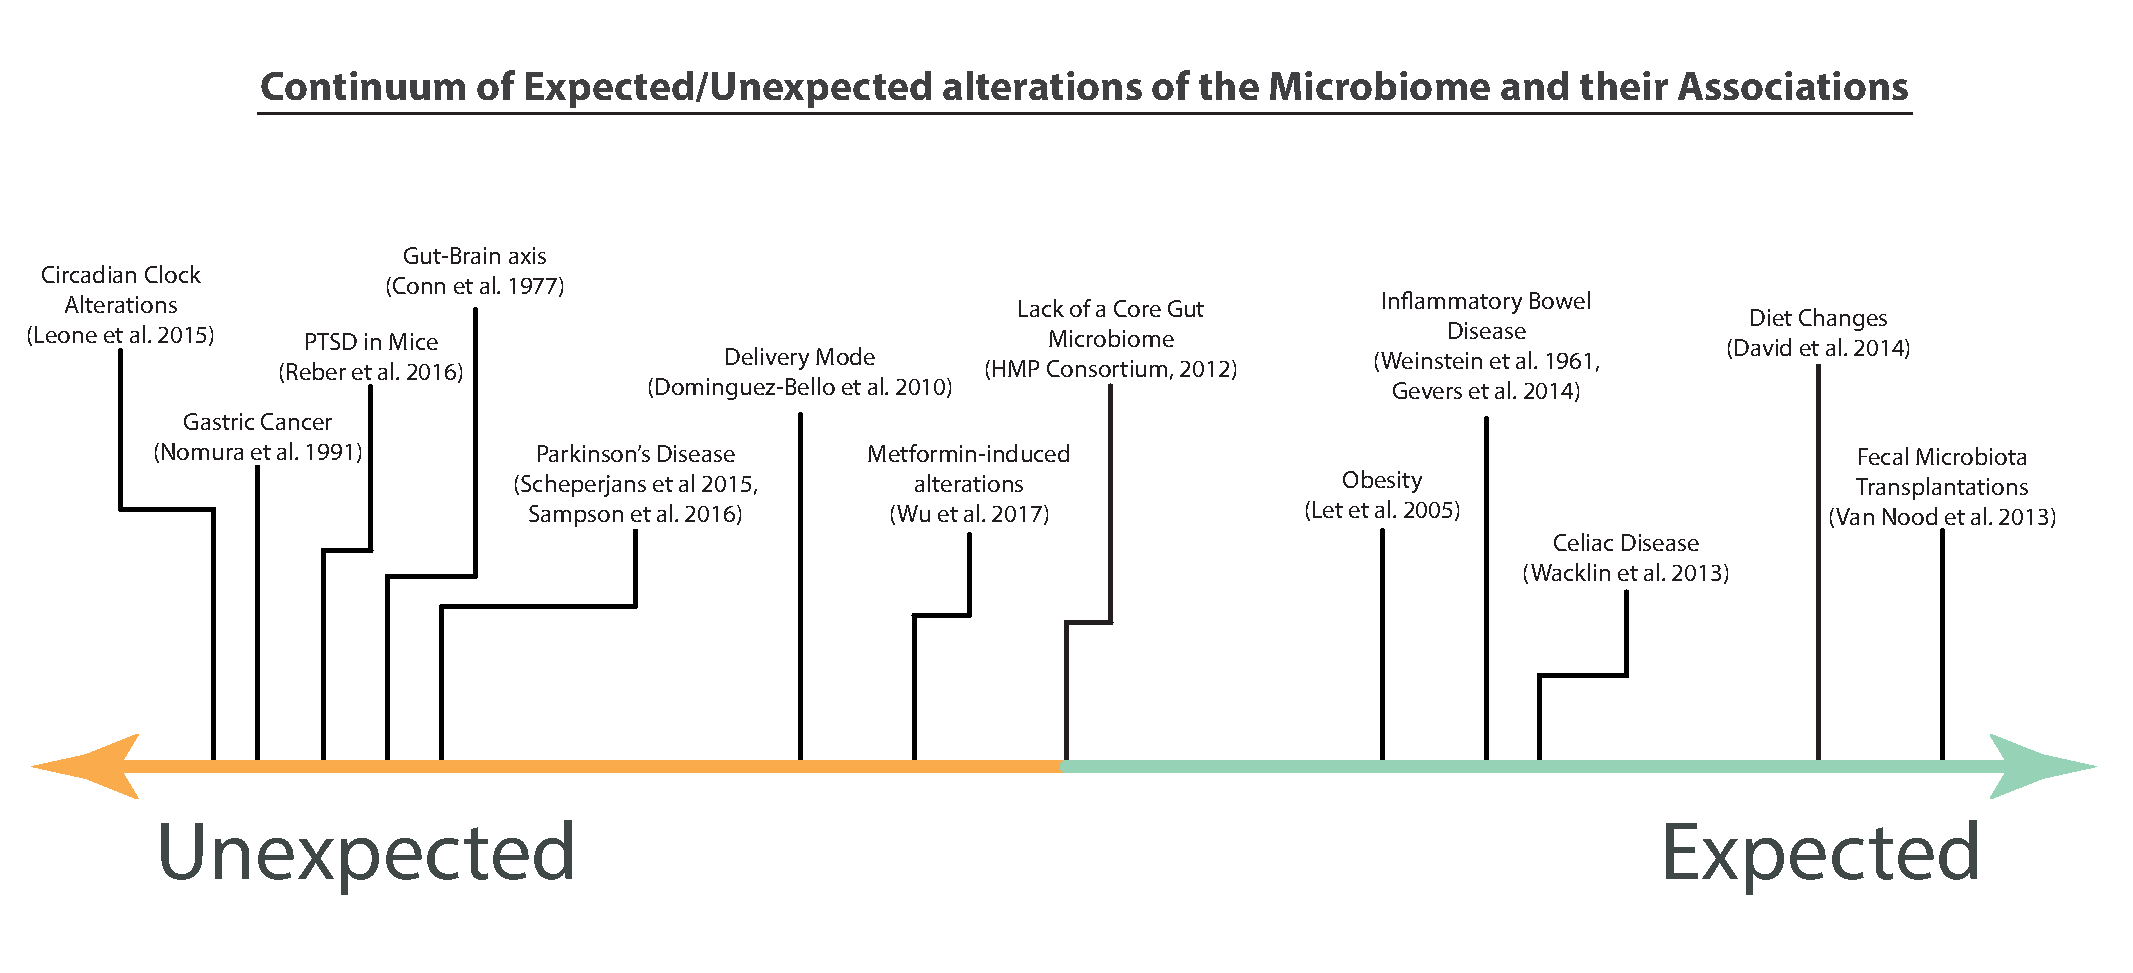
\includegraphics[width=0.95\textheight]{review-figures/figure-1}
\label{review_fig1}
\caption[A list of associations between the gut microbiome and various phenotypes]{A list of associations between the gut microbiome and various phenotypes, ranked by how expected or unexpected they were relative to previous knowledge [rank reflects consensus opinions of the co-authors of this Review, motivated by Figure 1 in \cite{RN4058}]}
\end{sidewaysfigure}


In this review, we focus on the human gut microbiome, although, where appropriate, we refer to studies using animal models, especially gnotobiotic mice (germ-free mice colonized with a defined set of microbes, either pure strains or fecal material from a rodent or human donor). As noted above, different parts of the human body (e.g., mouth, skin, airways, and urogenital tract) have distinct microbiomes from the gut microbiome, but the gut has been most studied in terms of drug response, in part because it contains by far the greatest microbial biomass in the human body, and therefore, the greatest capacity for drug metabolism. We first provide an overview of the diversity of the human gut microbiome, identifying key factors that structure the microbiome in healthy and diseased populations. We then describe connections between gut microbes and the action of several therapeutic agents, ranging from antibiotics to analgesics. Third, we describe how the microbiome can alter host response to drugs, though not necessarily metabolizing the drugs themselves. Fourth, we discuss prospects for identifying which patients will respond to a given drug based on the whole microbiome and prospects for exploiting the microbiome as a companion diagnostic to increase efficacy or reduce adverse events. Finally, we provide an outlook for the field in terms of improved patient stratification, and raise the intriguing prospect that patients might be converted from non-responders to responders via the use of companion therapies that alter the microbiome to increase efficacy of a specific drug.


\section{Diversity of the human gut microbiome across populations and life stages}

There are very few germ-free humans; therefore, understanding differences among individuals colonized with different microbes is key for predicting those who will respond similarly to drugs. However, many of the factors affecting the microbiome are highly counterintuitive. Here we focus primarily on a recent review \cite{RN4057}, five large-scale studies \cite{RN4108, RN4104, RN4107, RN4061, RN4059}, and two large-scale meta-analyses \cite{RN4062, RN4063} that summarize these findings.

As noted above, different sites in the human body host highly distinct microbial communities: on a Principal Coordinates Analysis `map' of the microbiome, they emerge as different `continents' \cite{RN4066, RN4107}. However, the differences in microbiome composition between, for example, the mouth and the gut of the same person are much greater than the differences between soil samples collected from different continents, and instead are more comparable to the difference between soil and seawater \cite{RN4087}. Although different body sites are highly distinct at the level of microbial taxa, they are relatively similar in terms of major microbial metabolic functions, at least as measured by \gls{kegg} pathways or other broad levels of gene function \cite{RN4107, RN4044}.

This pattern of microbial biogeography extends to the human gut \cite{RN4065, RN4066, RN4048, RN4070}. The microbiome changes dramatically along the gastrointestinal tract, with distinct populations in the oral cavity, esophagus, stomach, and small and large intestine. The most abundant genera of the oral cavity include \textit{Actinomyces}, \textit{Streptococcus}, \textit{Neisseria}, and \textit{Veillonella}, while the throat and stomach are dominated by \textit{Streptococcus} and \textit{Prevotella} species. In the stomach, roughly half of individuals are colonized by \textit{Helicobacteria pylori}, which dominates the gastric microbiome in these individuals \cite{RN4071}. The small intestine harbors fast-growing, G+C rich organisms specialized in digesting simple carbohydrates \cite{RN4067} and is often dominated by genera such as \textit{Peptostreptococcus}, which are rare in the large intestine. The bulk of the microbiome and microbial metabolism is in the large intestine. Typical bacterial loads are 105~CFU/ml in the jejunum, 106~CFU/ml in the ileum, but 108~CFU/ml in the cecum \cite{RN4110}, and 1011-1012~CFU/g in the feces \cite{RN4068}. This, together with stool being a relatively good proxy for the large intestine luminal contents but much more convenient to sample, means that most attention has focused on stool. However, for some applications such as detecting inflammatory bowel disease, microbiome analyses from biopsies dramatically outperform analyses of stool in their ability to distinguish healthy from diseased subjects \cite{RN4069}. The range of study designs where biopsies are essential is still hotly debated; nonetheless, stool biomarkers are highly informative for many applications, as noted below.

The process of development from infancy to early childhood has the greatest known effect on the stool microbiome. This effect is so profound that it traverses the vast gulf in microbiome configuration among body sites (Figure~\ref{review_fig2}). As they pass through the birth canal, newborns are typically colonized by bacteria resembling the constituents of the mother’s vaginal microbiome. By contrast, newborns delivered by C-section without labor lack these co-evolved vaginal microbes. Instead their microbiome resembles the skin, either from direct contact with caregivers and medical staff or from dust, which largely consists of human skin flakes and their associated microbes in indoor environments \cite{RN4115, RN4116, RN4118}. The first few weeks of life are chaos in the infant gut microbiome \cite{RN4120, RN4119} with very large differences at successive time points and among children. The subsequent overall process of development to the adult state takes about 2-3 years \cite{RN4115, RN4120, RN4061}, although smaller changes continue throughout childhood \cite{RN4061}. Intriguingly, although the process of development to the adult state is consistent cross-culturally, the state that is reached varies across populations \cite{RN4061}. These major differences in the microbiome may explain some of the differences in drug response between children and adults that are not explained by other factors.

\begin{figure}[htbp]
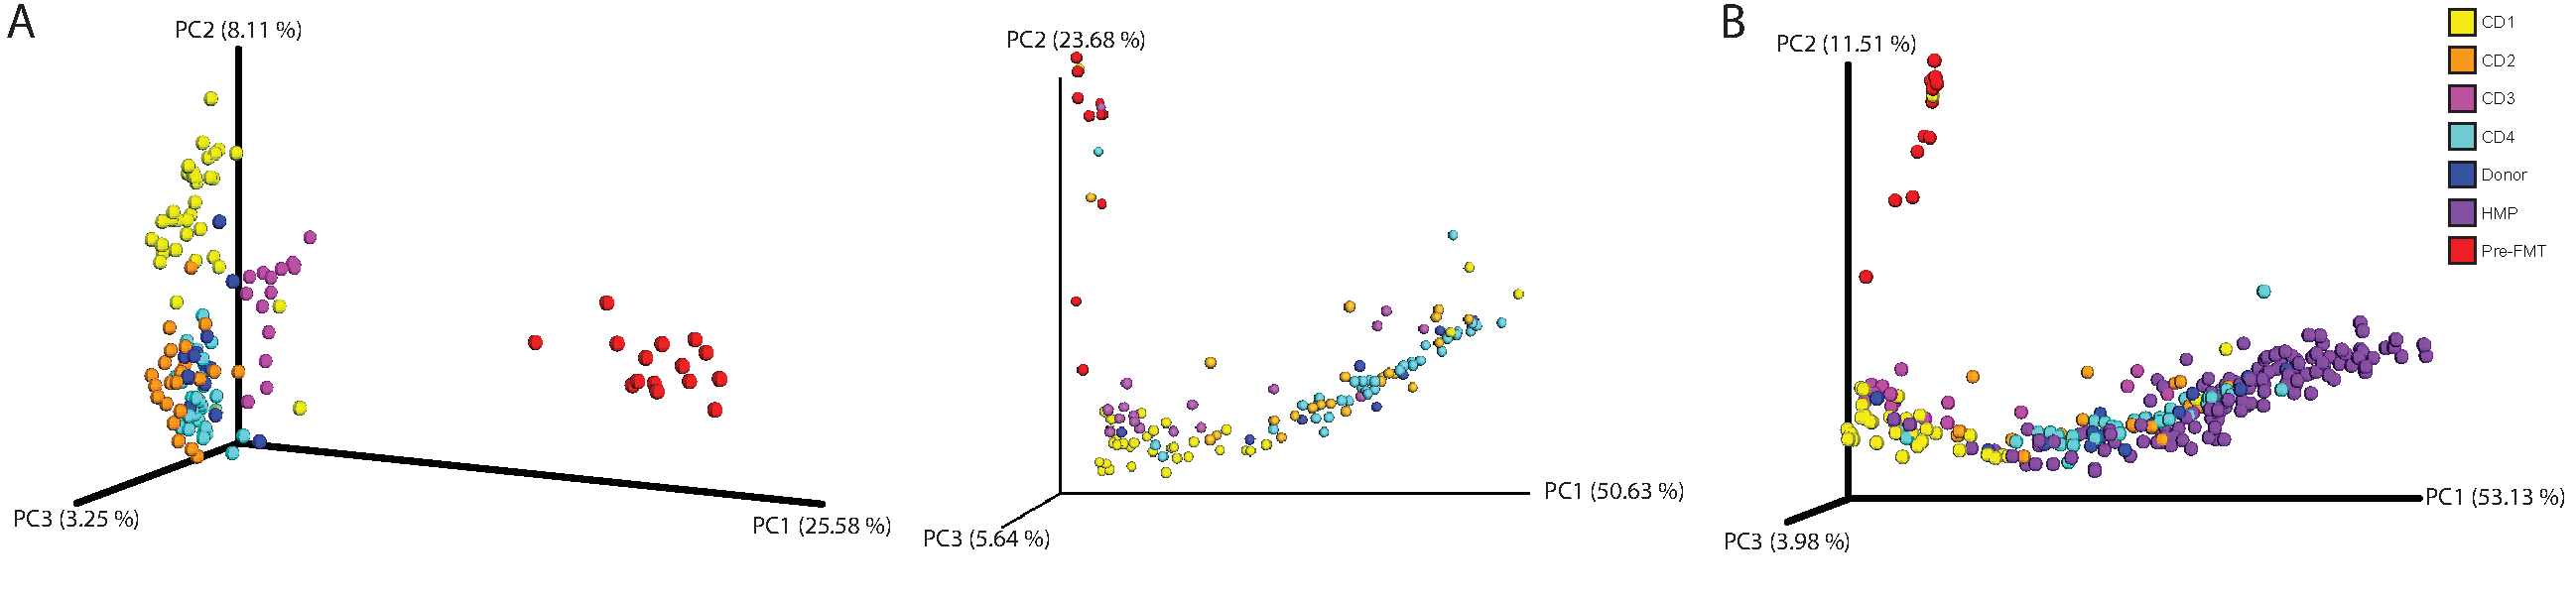
\includegraphics[height=0.65\textheight]{review-figures/figure-2}
\label{review_fig2}
\caption[Principal coordinates analysis on unweighted UniFrac distances of the process of microbiome assembly in the gut of one infant, contextualized with the Human Microbiome Project.]{Principal coordinates analysis on unweighted UniFrac distances of the process of microbiome assembly in the gut of one infant, contextualized with the Human Microbiome Project. Panel (A) colored by the sample type, and (B) colored by infant's age. As time goes by, the microbial communities in the infant's stool shift from resembling healthy adult vaginal and skin communities to resemble stool composition. This demonstrates how the process of gut microbiome development spans some of the most profound changes in the microbiome, i.e. the distance across different body sites.}
\end{figure}

Drugs that work in one human population may fail for unknown reasons in other populations, though the reasons for this are often obscure. Large efforts (and amounts of money) have sought the answer by studying human genomes. However, human genomes are 99.9\% the same but gut microbiomes can be 90\% different \cite{RN4081}. Given the rate of microbial metabolism and diversity of microbially-encoded enzymes, it makes sense to inquire whether  differences in drug responses are linked to the gut microbiome. Indeed, different human populations have markedly different microbiomes, which are largely thought to be linked to diet, with an axis that trades \textit{Prevotella} in diets rich in sugar and grains for \textit{Bacteroides} in diets rich in animal protein. These trends have been observed in the US population \cite{RN4088} and among US, South American, and African populations \cite{RN4061}. However, diet cannot be the sole driver, or between-population microbiome variation would not exceed the within-population variation, yet this is what one observes.

Even with hundreds of individuals, it is not yet possible to ascertain the factors at the population level that are most important in structuring the adult gut microbiome, because diet, environmental (including drug) exposures, host genetics, and other factors vary among populations in complex ways. Studies encompassing dozens of populations, with detailed tracking of individual- and population-level information, are likely required to resolve these questions, just as for such questions in human population genetics \cite{RN4078}. Hunter-gatherer populations, such as the Yanomami in the Amazon basin and the Hadza in sub-Saharan Africa, have distinct microbiomes harboring entire phyla, such as Spirochetes, that are even absent from rural farming populations \cite{RN4111, RN4113, RN4112}. This suggests that the loss of diversity from the microbiome of modern populations may have begun with the advent of agriculture. However, other factors such as C-section, antibiotics, and hygiene practices may be leading to continual depletion of our natural microbial symbionts \cite{RN4079}.

Several population-based studies that examine many variables have begun to provide insights into factors that shape microbiomes within populations. Drugs, especially antibiotics, but also metformin and proton pump inhibitors, have a surprisingly large effect on the microbiome and must be controlled for in studies that seek to link microbiomes to disease \cite{RN4080}. Long-term diet has a large effect, especially the balance of carbohydrates and protein. Age and season have large effects, although it is not known whether these are mediated in part by diet. Having a dog has an intermediate effect, smaller in the gut than in the skin and in the indoor environment \cite{RN4083, RN4082}. Many other factors, including sex, \gls{bmi}, and even amounts of sleep and exercise can be identified as differences among groups that contain hundreds of subjects per group but cannot be used to classify individuals. Host genetics has a surprisingly small impact in humans compared to other factors: although monozygotic twins are slightly more similar to one another than are dizygotic twins, hundreds of twin pairs are needed to see this effect. However, some specific components of the microbiome are highly heritable and correlate with phenotype. For example, Christensenella, identified by microbiome-wide heritability analysis, correlated with low \gls{bmi}, including in slimmed down germ-free mice that received an otherwise obesogenic microbiome from an obese human donor. Replicating this feat to manipulate weight or other phenotypes in humans remains a goal for future studies.

\section{Connections between specific gut microbes and action of therapeutic agents}
  
The literature demonstrating how gut microbes affect the efficacy or toxicity of specific drugs is expanding rapidly. Here we provide a few illustrative examples see also Table~\ref{review_tab1} for a brief summary. For additional examples, readers should  consult recent reviews \cite{RN4084,RN4086}.

\subsection{Analgesics}
\Glspl{nsaid} are used for pain relief in many conditions. Multiple studies have demonstrated that \gls{nsaid} use is associated with damage to the small intestine; the severity of this damage depends on the microbial community present at the time of \gls{nsaid} administration \cite{RN4107, RN4109}. Increased Gram-negative taxa have been associated with more severe damage \cite{RN4109, RN4124}. However, the precise link between \gls{nsaid}-induced damage and the microbiome remains poorly understood. Antibiotic treatment can alter the existing microbial community enough to reduce \gls{nsaid}-associated small intestinal damage in humans \cite{RN4085}, and can alter microbial metabolism of aspirin to potentiate its anti-thrombotic effects in mice \cite{RN4090}. However, other known negative effects of antibiotic treatment suggest risks in using antibiotics to reduce adverse events from specific combinations of microbiome state and \gls{nsaid} use. For example, antibiotic treatment of mice transplanted with a microbiome considered to be `protective' against \gls{nsaid} damage produced higher mortality with \gls{nsaid} administration \cite{RN4089}, underscoring that the association between \gls{nsaid} usage, microbiome community structure, and bowel damage reduction is complex and must be approached carefully. Probiotic strains have been deployed to prevent \gls{nsaid}-induced bowel damage. For example, protective effects of \textit{Lactobacillus gasseri} against aspirin-induced small intestinal damage have been assessed in human subjects \cite{RN4091}, and although results were promising, studies in larger populations are needed to evaluate the efficacy of this approach. In addition, the impact of the gut microbiome on the bioavailability, efficacy and toxicity of orally administered drugs, xenobiotics and dietary substances was studied for $>$30 pro-drugs \cite{RN4136}. Many prodrugs that treat gut inflammation are converted to active forms by the gut microbiome. These include sulfasalazine, olsalazine, ipsalazide and balsalazide, for which the aminosalicylic acid needs to be released in order to become active \cite{RN4093}. Gut bacteria of the genera Clostridia and Eubacteria exhibit this ability \cite{RN4094}.

\subsection{Antibiotics}
Although antibiotics influence the composition of the microbiome, the effects of antibiotic treatment depend on its starting composition. The extent of cellular damage induced by ex vivo antibiotic exposure of fecal samples depends on the individual's original microbiota \cite{RN4095}. This is consistent with previous data demonstrating species-specific susceptibility to antibiotics \cite{RN4096}. Healthy adults with similar microbial communities prior to treatment with cefprozil had similar alterations in the abundance of \textit{Enterobacter cloaceae} following treatment \cite{RN4097}. The gut microbiome may also regulate the effect of antibiotics at distal sites of infection. Resistance genes that lead to chemical modifications, such as hydrolysis or chemical modification, may decrease the bioavailability of the antibiotic \cite{RN4098}, potentially leading to a lower effective concentration at the primary site of infection. Future work is needed to investigate whether the overall gut microbiome composition influences these resistance genes.

\subsection{Cardiac glycosides}
Cardiac glycosides are a family of organic compounds that increase the contractility of the heart and are prescribed mainly for congestive heart failure and cardiac arrhythmia. The bioavailability of one of the most common cardiac glycosides, digoxin, varies greatly among patients. Early experiments showed that some patients’ gut microbiota can metabolize digoxin into inactive metabolites and that pretreatment with antibiotics in individuals harboring these microbiota increased the plasma level of digoxin \cite{RN4099}. Detailed metagenomic analysis identified a \gls{cgr} operon in some, but not other, strains of the commensal gut bacteria \textit{Eggerthella lenta}, which is responsible for the degradation of this drug \cite{RN4102}. Studies in animal models revealed that supplementation with the amino acid arginine can suppress the cgr operon and increase digoxin bioavailability. These experiments underline the importance of the microbiome in drug metabolism and provide an example where targeted therapeutic alternatives, in this case arginine supplementation in place of antibiotic treatment, can improve clinical outcomes.

\subsection{Metformin}
Metformin is used in the treatment of \gls{t2d}. Since its introduction in the 1950s \cite{RN4103}, many mechanisms of action have been proposed to explain its effects on the liver and insulin-sensitive tissues \cite{RN4126}. However, a recent report of trans-species transmission of the therapeutic effect of improved glucose tolerance from the stool of metformin-treated humans into germ-free mice \cite{RN4127} suggests that the insulin-sensitizing effects of the drug may result from a metabolic shift in the gut microbiome rather than direct effects on the liver or other tissues. Further evidence for this mechanism is suggested by the fact that most common side-effects of metformin are GI-centric (nausea, vomiting and diarrhea), and delivery of metformin into the portal vein did not change hepatic glucose production \cite{RN4128}.

\subsection{Fecal microbiota transplants (FMT)}
Microbiome transplants could potentially be used for many indications in the gut, but also in skin, oral, eye and vaginal health. The most prominent example is the treatment of recurrent \gls{cdi}. The standard of care for recurrent \gls{cdi} is antibiotics, which inadvertently deplete other microbes necessary for healthy gut function. \Gls{fmt} have outstanding efficacy in treating \glspl{cdi} \cite{RN4129}. The procedure relies on finding a healthy donor (often a close-relative or friend, although the evidentiary basis for this choice is weak), who donates fecal microbes for transplant into the diseased subject. Changes occur in the microbial communities of the recipient in less than a day, and disease-associated symptoms quickly disappear \cite{RN4130}. A meta-analysis of longitudinal datasets revealed that post-FMT subjects also recover dynamic features common to healthy humans \cite{RN4131}. \Glspl{fmt} are not 100\% effective and there is even anecdotal evidence of unintended changes, such as sudden excessive weight gain post-\gls{fmt} \cite{RN4132}. This has led researchers to seek optimal conditions for effective \gls{fmt}, such as antibiotic pre-treatment \cite{RN4134, RN4133}. From an ecological standpoint, the logic behind this is straightforward, because newly introduced communities need not compete with an established community of bacteria, and can develop interactions likely already present in the donor's gut. Outside the gut, adding microbes from healthy individuals to skin afflicted with atopic dermatitis reduces symptoms \cite{RN4135} and vaginal microbe transplants from healthy individuals may overcome bacterial vaginosis [clinical trial\footnote{\url{https://clinicaltrials.gov/ct2/show/NCT02236429}}]. The microbiome field is still young so other beneficial transplant therapies will likely be developed in the future. However, public enthusiasm for such treatments and for probiotics still greatly outstrips the available scientific evidence.

\begin{sidewaystable}[htbp]
\centering
\caption[Summary of selected studies where the microbiome is known to be implicated in the outcome of a treatment.]{Summary of selected studies where the microbiome is known to be implicated in the outcome of a treatment. In these cases, the presence or absence of a group of bacteria may hinder or promote the efficacy of a procedure}
\label{review_tab1}
\renewcommand{\arraystretch}{0.8}% Tighter
\scalebox{0.95}{\begin{tabular}{p{6cm}p{14cm}P{2cm}}
\toprule
Treatment &	Interaction	& Reported\\
\midrule
Non-steroidal anti-inflammatory drugs (NSAIDs) & 	Increased gram negative bacteria are associated with increased damage to the small intestine. These lesions can be ameliorated if pre-treated with antibiotics &	\cite{RN4124,RN4085}\\
Antibiotics & Treatment effect depends on the host's starting composition and antibiotic class. Subjects with similar profiles had correlated abundance alterations of Enterobacter \textit{cloaceae}. & \cite{RN4095,RN4097}\\
Cardiac Glycosides & The bioavailability of digoxin is affected by the presence of \textit{Eggerthella lenta}, this can be regulated by suppressing the reductase responsible for degrading this drug. & \cite{RN4099,RN4102}\\
Metformin & The mechanism driving the effect of this drug is a result of metabolic shifts of the gut microbiome. &	\cite{RN4127}\\
Fecal Microbiome Transplant &	The efficacy of this treatment is known to benefit from pre-treatment with antibiotics. & \cite{RN4134,RN4133}\\
Chemotherapeutics & Negative drug-drug interactions by bacterial metabolism, protection from chemotherapy-related bloodstream infection.& \cite{RN4225,RN4226}\\
\bottomrule
\end{tabular}}
\renewcommand{\arraystretch}{1}% Restore original value
\end{sidewaystable}

\section{Microbiome effects on host responses to drugs}
An important emerging area of investigation in drug response is the effects of the microbiome on host responses to chemotherapeutics. Although sequencing tumors and pharmacogenomics plays a key role in precision medicine, our microbial genomes can also affect host gene expression throughout the body, altering drug metabolism and efficacy. Because the gut microbiome varies markedly among individuals, host-drug interactions mediated by microbial metabolism warrant close consideration in tailoring patient treatment.

Studying drug `co-metabolism' by the gut microbiota and the human host is complicated by interindividual variability in human genetics, diet, and other clinical factors. Additionally, the human intestine is relatively inaccessible for direct examination. Animal and in vitro models can provide useful tools to simplify the study of these interactions. Even non-mammalian models can be important for exploring drug metabolism. For example, fluropyrimidines are among the most widely used chemotherapeutics for treating colon cancer. Two detailed mechanistic studies exploiting the power of large population sizes in \textit{C. elegans} combined with the ability to associate specific components of the microbiome and mutant bacterial strains allowed elucidation of the precise pathways by which components of the microbiome such as \textit{E. coli} and \textit{Comamonas upp} enable the action of this chemotherapeutic agent via bacterial pyrimidine metabolism, using proliferation of gonad cells (and hence reproduction) as a bioassay for side-effects \cite{RN4101, RN4100}. This is a new innovation as mammalian (mouse, rat, guinea pig, hamster, rabbit) models are more widely used to study the interaction of microbial communities and common pharmaceuticals. 

Although human studies are the gold standard, they have many limitations. They require \gls{irb} approval, are invasive, costly, and there is high and uncontrolled inter-individual variability. Close medical supervision is required and toxicity must be carefully monitored. Animal studies are less expensive, have logistical advantages with control of age and dietary variability, and all tissues can be directly accessed. However, the results do not always translate to humans (in part because the gastrointestinal physiology, diet and microbiome all differ markedly) and coprophagy can be an issue. Even so, animal studies have considerable cost and ethical issues, especially when large sample sizes are needed to set dosage ranges and identify sources of inter-individual variability. In vitro systems are therefore attractive models and preferred in early preclinical phases of drug discovery and screening. They are cheaper and  provide easy access to materials, logistical and scale advantages, and incur no ethical concerns \cite{RN4136}. However, in vitro systems are often oversimplified and lack intestinal secretion, measures of absorption, and host-microbe interactions. Nonetheless, several in vitro models have been developed and have had considerable utility. One is a \gls{shime} consisting of a six-stage reactor, simulating stomach, duodenum/jejunum, ileum, ascending, transverse and descending colon \cite{RN4137} and provides a simpler model for growing human fecal bacteria at scale \cite{RN4138}. Each experimental method has its own advantages and disadvantages; in vivo studies provide insight in the real life colonic metabolism, while in vitro models are more cost-effective and do not have ethical drawbacks. No perfect model exists and therefore a combination of different methods is preferred to clarify the role of the gut microbiome in drug metabolism. 

Diet can modify the gut microbiome and gene expression of the host and thus influence epigenetic changes associated with diseases; such changes affect host gene expression through histone modifications, DNA methylation and non-coding RNAs \cite{RN4139}. The epigenetic changes are heritable and persist from one cell generation to the next. Nutrition contributes to a large extent to the gut microbiome and the gut microbiome has an important role in human metabolism. The gut microbiome is thus potentially the largest environmental factor affecting the human epigenome. Indeed, comparisons of germ-free mice with conventionally raised mice show differences in gene expression patterns throughout the body, including in the liver and brain. Initially germ-free mice colonized early with microbes resembled conventionally raised mice in physiology, gene expression and behavior, whereas those colonized later resembled germ-free mice, suggesting microbiome-mediated critical periods for development \cite{RN4140}. However, the mechanistic basis for these effects is unknown. One specific interaction that has been well characterized is that bacteria are responsible for short chain fatty acid formation, especially butyrate, in the gut. Butyrate promotes cell turnover of colon epithelium cells. In colonic cancer cells, glucose rather than butyrate is used as growth substrate. Butyrate accumulates in the nucleus, inhibits cell proliferation and induces cell apoptosis \cite{RN4141}. In addition to their impact on the colonic epithelium, many microbial products are absorbed into the blood and lymph and can alter gene expression systemically. 

In the human body small-molecule drugs are largely metabolized by human cytochrome P450 enzymes in the liver (CYP450). These enzymes can also convert prodrugs into their active molecules. P450 enzymes are highly polymorphic in humans and greatly impact drug response \cite{RN4142}. The variability in CYP450 is not limited to humans: bacterial CYP450 enzymes vary in copy number, function, and substrate \cite{RN4143}. Germ-free mice have different CYP450 expression profiles than conventionally raised mice and alterations in expression of other host genes linked to xenobiotic metabolism \cite{RN4144}. Although differences in the microbiome have not been linked to CYP450 activity in humans, accurate prediction of drug metabolism may ultimately require knowledge of both human CYP and the gut microbiota genetics, since one of the functional roles of the gut is to partially digest and absorb nutrients and therefore is a major component of metabolismi. Microbially-encoded cytochromes can also be directly important for drug metabolism. For example, as noted above, a classic example of microbiota-drug interactions is inactivation of the cardiac glycoside digoxin by \textit{Eggerthella lenta} \cite{RN4099} with metabolism by  the cytochrome-encoding cgr operon in strains of \textit{E. lenta} \cite{RN4146}. 

Bile acids are produced by hepatocytes and released by the gall bladder into the duodenum to absorb fatty acids, cholesterol, and fat-soluble compounds \cite{RN4147}. They are highly efficient detergents that digest, solubilize, and absorb dietary lipids and vitamins, and are widely used in drug delivery systems with increasing interest in using them directly as therapeutic agents \cite{RN4148}. Bile acids are metabolized by the gut microbiota into secondary bile acids \cite{RN4149}, which  are reabsorbed  via the enterohepatic circulation and again back into the liver, biliary tract and gut. The gut microbiome not only influences secondary bile acid formation in gut but also modulates the enterohepatic system by regulating the bile acid synthesis in the liver \cite{RN4150}. High levels of secondary bile acids are linked to gastrointestinal diseases, colon cancer and gallstones \cite{RN4152}. For example, a meat-based diet is associated with higher levels of taurine conjugation to bile acids and gut production of hydrogen sulfide \cite{RN4153}, which can lead to colon cancer. A high intake of saturated fats leads to a higher abundance of Clostridium clusters XI/XIVa and sulfate- or sulfite-reducing bacteria, which are linked to an increase in secondary bile acids produced by the microbiota \cite{RN4154}. Similarly the gut microbiome can contribute to obesity and type 2 diabetes since lipid and glucose metabolism are regulated by secondary bile acids in the gut \cite{RN4155}. Considerable potential exists for using probiotics to reduce the levels of specific secondary bile acids in the colon, although clinical trials and validated outcomes are still lacking. In vitro models have shown the potential of lactobacilli and bifidobacteria to assimilate cholic acid in their cells \cite{RN4156}. Thus modifying secondary bile acid production by modifying the microbiome  has promise, although validation in humans is yet to be established.

\section{Prospects for stratifying patient response based on the whole microbiome}

The considerable interindividual variation of the gut microbiome, together with the impact of the microbiome on drug metabolism opens up possibilities for stratifying patients on the basis of predicted response to a given intervention. 

Microbiome studies, including stratification, have been dramatically transformed by computational tool development \cite{RN4160, RN4161, RN4158, RN4159, RN4157}. Most developments address only a specific problem within a long sequence of steps. Tools such as \gls{qiime} (Quantitative Insights Into Microbial Ecology) \cite{RN4052} provide an integrated platform that allows scientists to go directly from DNA sequences to actionable and interpretable results. More recently these platforms  are available in the form of web applications (MG-RAST \cite{RN4162}, MicrobiomeAnalyst \cite{RN4163}, VAMPS \cite{RN4164}, Qiita\footnote{\url{https://qiita.ucsd.edu/}}. Such integrated platforms allow analysis and storage of microbiome data and reduce infrastructure problems such as storage, data deposition and fault tolerance. These challenges must be overcome even for small microbiome studies.

These microbiome analytic platforms have been used to look for differences in the microbiome and to stratify patients in terms of their therapeutic response in a number of diseases. For example, \gls{ibd}, a gastrointestinal autoimmune condition, has a history \cite{RN4172} and evidence supporting a microbial-driven origin or regulation \cite{RN4069, RN4175, RN4173}. In the studies cited, microbial and metabolic features were inferred from microbiome and metabolomic samples to distinguish between healthy and \gls{ibd}-affected subjects. This approach is of value because current diagnostic methods rely on expensive tests, such as the quantification of calprotectin present in fecal samples \cite{RN4177}. Further development of microbiome biomarkers could provide non-invasive, affordable methods to detect a group of bacteria or molecules. However, the classification accuracy of this method can be too low with fecal samples and even with rectal or ileal biopsies (which show the best performance) \cite{RN4069}. A promising approach uses a dog model of \gls{ibd} \cite{RN4179}, in which methods established and tested in humans were applied to a cohort of \gls{ibd} and non-\gls{ibd} affected dogs. In contrast to the sensitivity and specificity of the approach in humans, the microbial signal present in a dog’s fecal sample was sufficient to classify \gls{ibd} in dogs, with better performance than that obtained from biopsy samples in humans. These types of predictive models, using the microbiome data and certain data classifiers, have been useful for predicting which patients will best respond to specific drugs for Parkinson’s Disease \cite{RN4180}, and for predicting which dietary items have the greatest patient-specific impact on blood glucose response\cite{RN4181}.

Advances in untargeted metabolomics may be key for understanding microbial metabolism and its impact on drug responses. For \gls{ms}, the advent of large and community-curated reference knowledgebases like \gls{gnps} \cite{RN4182} provides a crowd-sourced data repository and peer-reviewed family of annotations for natural products, xenobiotics and metabolites. This is an important step towards the democratization and adoption of MS in a broad range of fields. \Gls{gnps} further provides an analytic infrastructure to help generate molecular networks \cite{RN4183} that can be used to study drug metabolism \cite{RN4184}. Integrating MS and microbiome data, whether 16S rRNA profiling or shotgun metagenomics, is not a simple task but will ultimately provide key insights into complex problems for which the microbial characteristics alone are not useful, and where, for example, the presence/absence of a molecule could break ties or strengthen inferences in an algorithmic context. Co-occurrence and co-exclusion detection models could potentially benefit, because the current state of the art presents formidable challenges \cite{RN4186, RN4185}. However, statistical obstacles must be addressed so as to improve the ability to  correlate microbiome and metabolite datasets. These dataset may have far more features than samples, and applying pairwise correlations leads to many spurious correlations. Finally, interpreting the results of these methods remains a major challenge, because these methods do not output correlations for individual microbiomes and molecules, but rather correlations between abstract axes that are composed of complex and often uninterpretable combinations of microbes and molecules. Enabling straightforward interpretation will be key for streamlining these methods so they can be applied clinically. Such interpretation will also become easier as \gls{ms} reference data and data sets of microbes and microbial molecules become available, a gap \gls{gnps} is aiming to fulfill.


\section{Outlook}
Recent advances have enabled the characterization of the human body from an integrative perspective across many data axes (`omes': genome, gene expression, microbiome, metabolome, virome, proteome, exposome, etc). When these heterogeneous data layers are combined, their full potential can address systems-level problems even when mechanisms are not fully understood. An outstanding example of this type of deep characterization is glycemic responses \cite{RN4181}:  by combining 16S rRNA microbial profiling, food frequency questionnaires, anthropometric data, and glucose monitoring, one can create a model that successfully predicts each individual’s blood glucose response to a specific meal and can create personalized diets that to increase or decrease the glycemic response of a set of new subjects not in the original study. These results are of utmost importance in this context, as the glycemic responses are known to be a personalized feature \cite{RN4192, RN4191}. In a separate study by the same group, researchers demonstrated that transitioning an individual's diet between industrial white bread, and whole grain sourdough bread, resulted in small changes in the microbiome and glycemic responses that differed on an individual-by-individual basis \cite{RN4193}. These experiments, which could be applied equally well to drug responses, are leading examples of the possibilities in the as-yet nascent ability to personalize treatments, not only based on the traditional one-dimensional approach (anthropometric data), but by modeling the body with a holistic integrative approach.

The microbes and molecules present on and in our bodies can produce a dysbiotic or healthy environment. Therefore, we must characterize the archetypical organizations of our microbiome in large populations. We caution against attractive yet incorrectly oversimplified stratification approaches \cite{RN4194} that are very sensitive to arbitrary parameter selections \cite{RN4195, RN4196}. Instead, one must embrace the complexity of the microbiome, including its dynamic features (for example the rate of change of groups of bacteria). It was recently shown that patients with active \gls{ibd} have microbiomes that experience more variability over time than healthy controls \cite{RN4197} while microbiome `motion' of healthy subjects was much more restricted. Properly establishing a mechanism that describes these dynamics and creating appropriate models that take them into account remains a challenge, given the number of patients and samples obtained longitudinally that will be required for validation.

Better models of drug action may require a microbiome component. In a large-scale study analyzing over 1,000 Dutch participants, a series of lifestyle descriptors (diet, smoking habits, medications, etc.) were used to model their bacterial composition, and these descriptors could recapture almost 20\% of the total microbial variation when using metagenomic sequences \cite{RN4059}. However, 80\% of variation remains unexplained. The microbiome may serve as a proxy to covariates that may not be readily available in all scenarios. For example, that study also found that decreased microbial and functional diversity was linked to a higher hemoglobin levels. Such studies need to unravel underlying mechanisms driving these associations and must show consistency across cohorts. 

Is it possible to change a patient4s microbiome to improve drug response?  An intriguing example of this is that bioavailability of the antiarrhythmic drug amiodarone can be increased by concomitant administration E. coli Nissle 1917 in rats \cite{RN4086, RN4201}. Similarly, in germ-free mice colonized with the \textit{Eggerthella lenta} DSM2243, access to a high protein diet rich in arginine inhibits digoxin inactivation \cite{RN4102, RN4202}, suggesting that dietary changes could also affect the metabolism of the native gut microbiota to modify efficacy. Cheaper microbiome sampling and analysis, combined with algorithms and visual displays to better interpret results, could therefore open up a whole new area of modifying or drugging the microbiome to convert drug non-responders into responders.

